\section{Neural Framework Analysis}

\subsection{Neural Approach Performance}

Neural network approaches to LRD estimation demonstrate potential advantages over classical methods through their ability to learn complex patterns and adapt to various data conditions. Figure \ref{fig:neural_framework} illustrates a framework comparison and performance characteristics.

\begin{figure}[h]
\centering
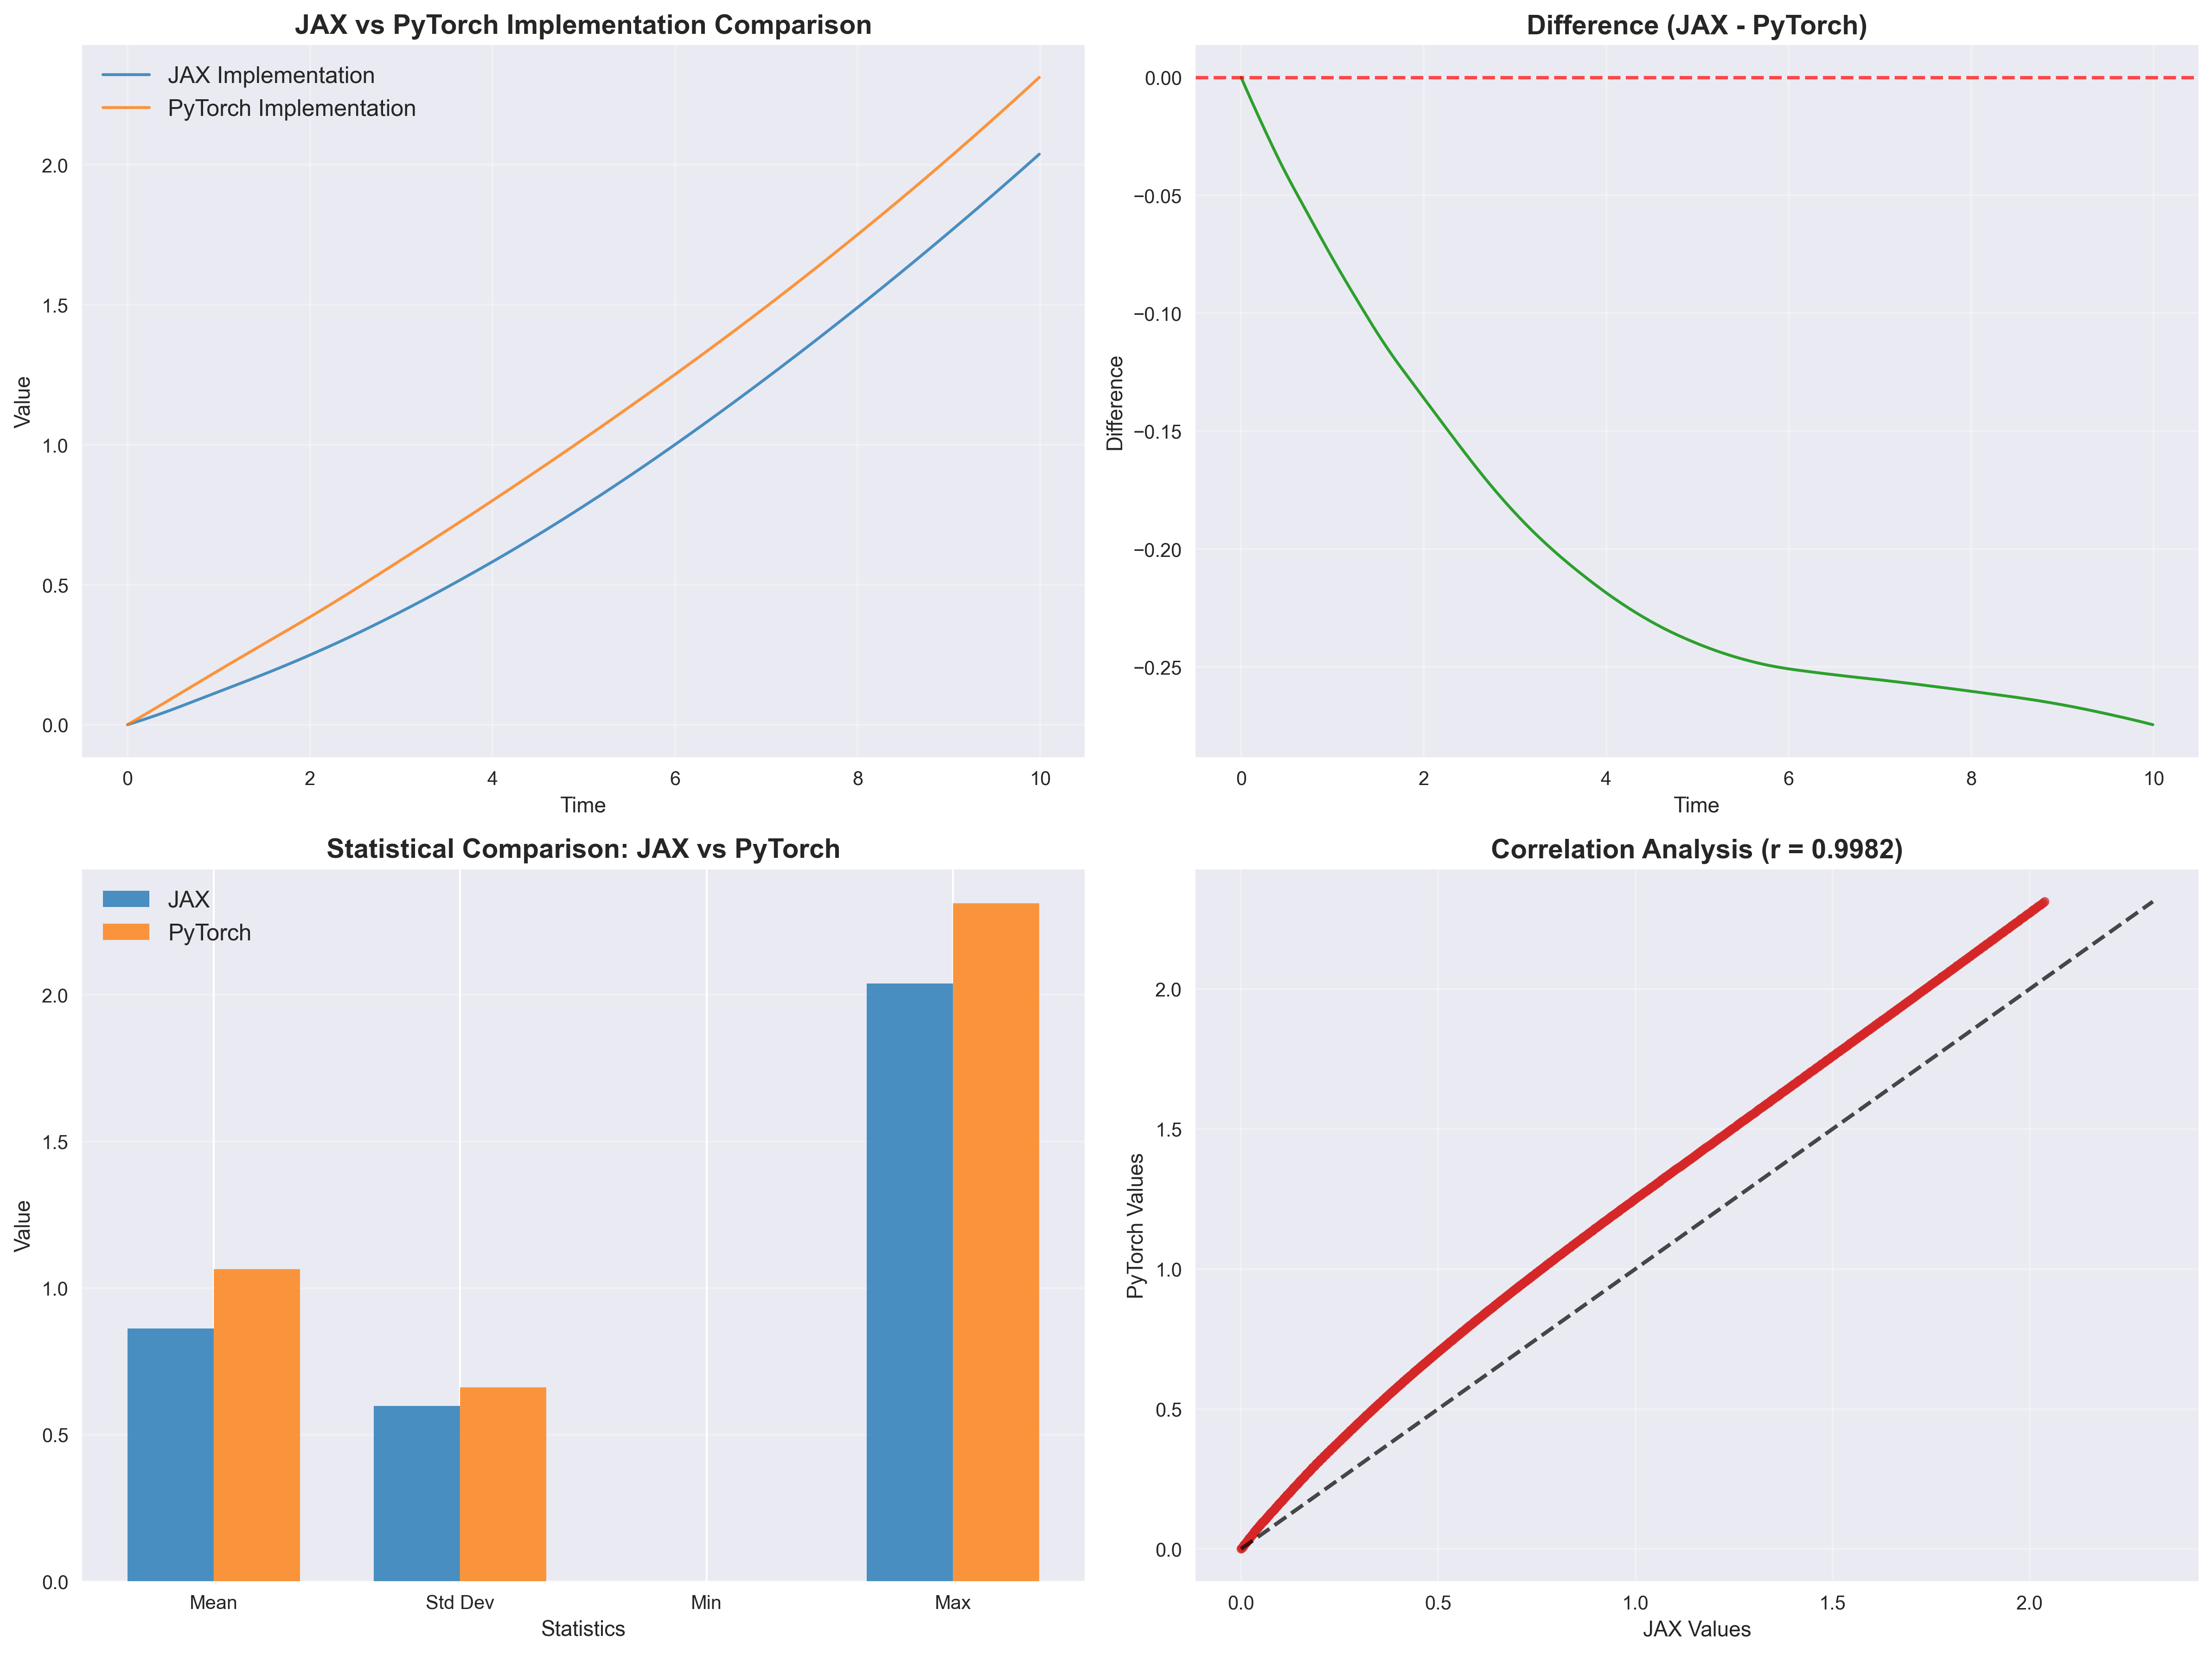
\includegraphics[width=0.8\textwidth]{neural_fsde_framework_comparison.png}
\caption{Neural Framework Comparison: Neural vs Classical Methods}
\label{fig:neural_framework}
\end{figure}

\subsection{Detailed Performance Analysis}

The detailed analysis reveals neural framework capabilities across different parameter ranges and data conditions:

\begin{figure}[h]
\centering
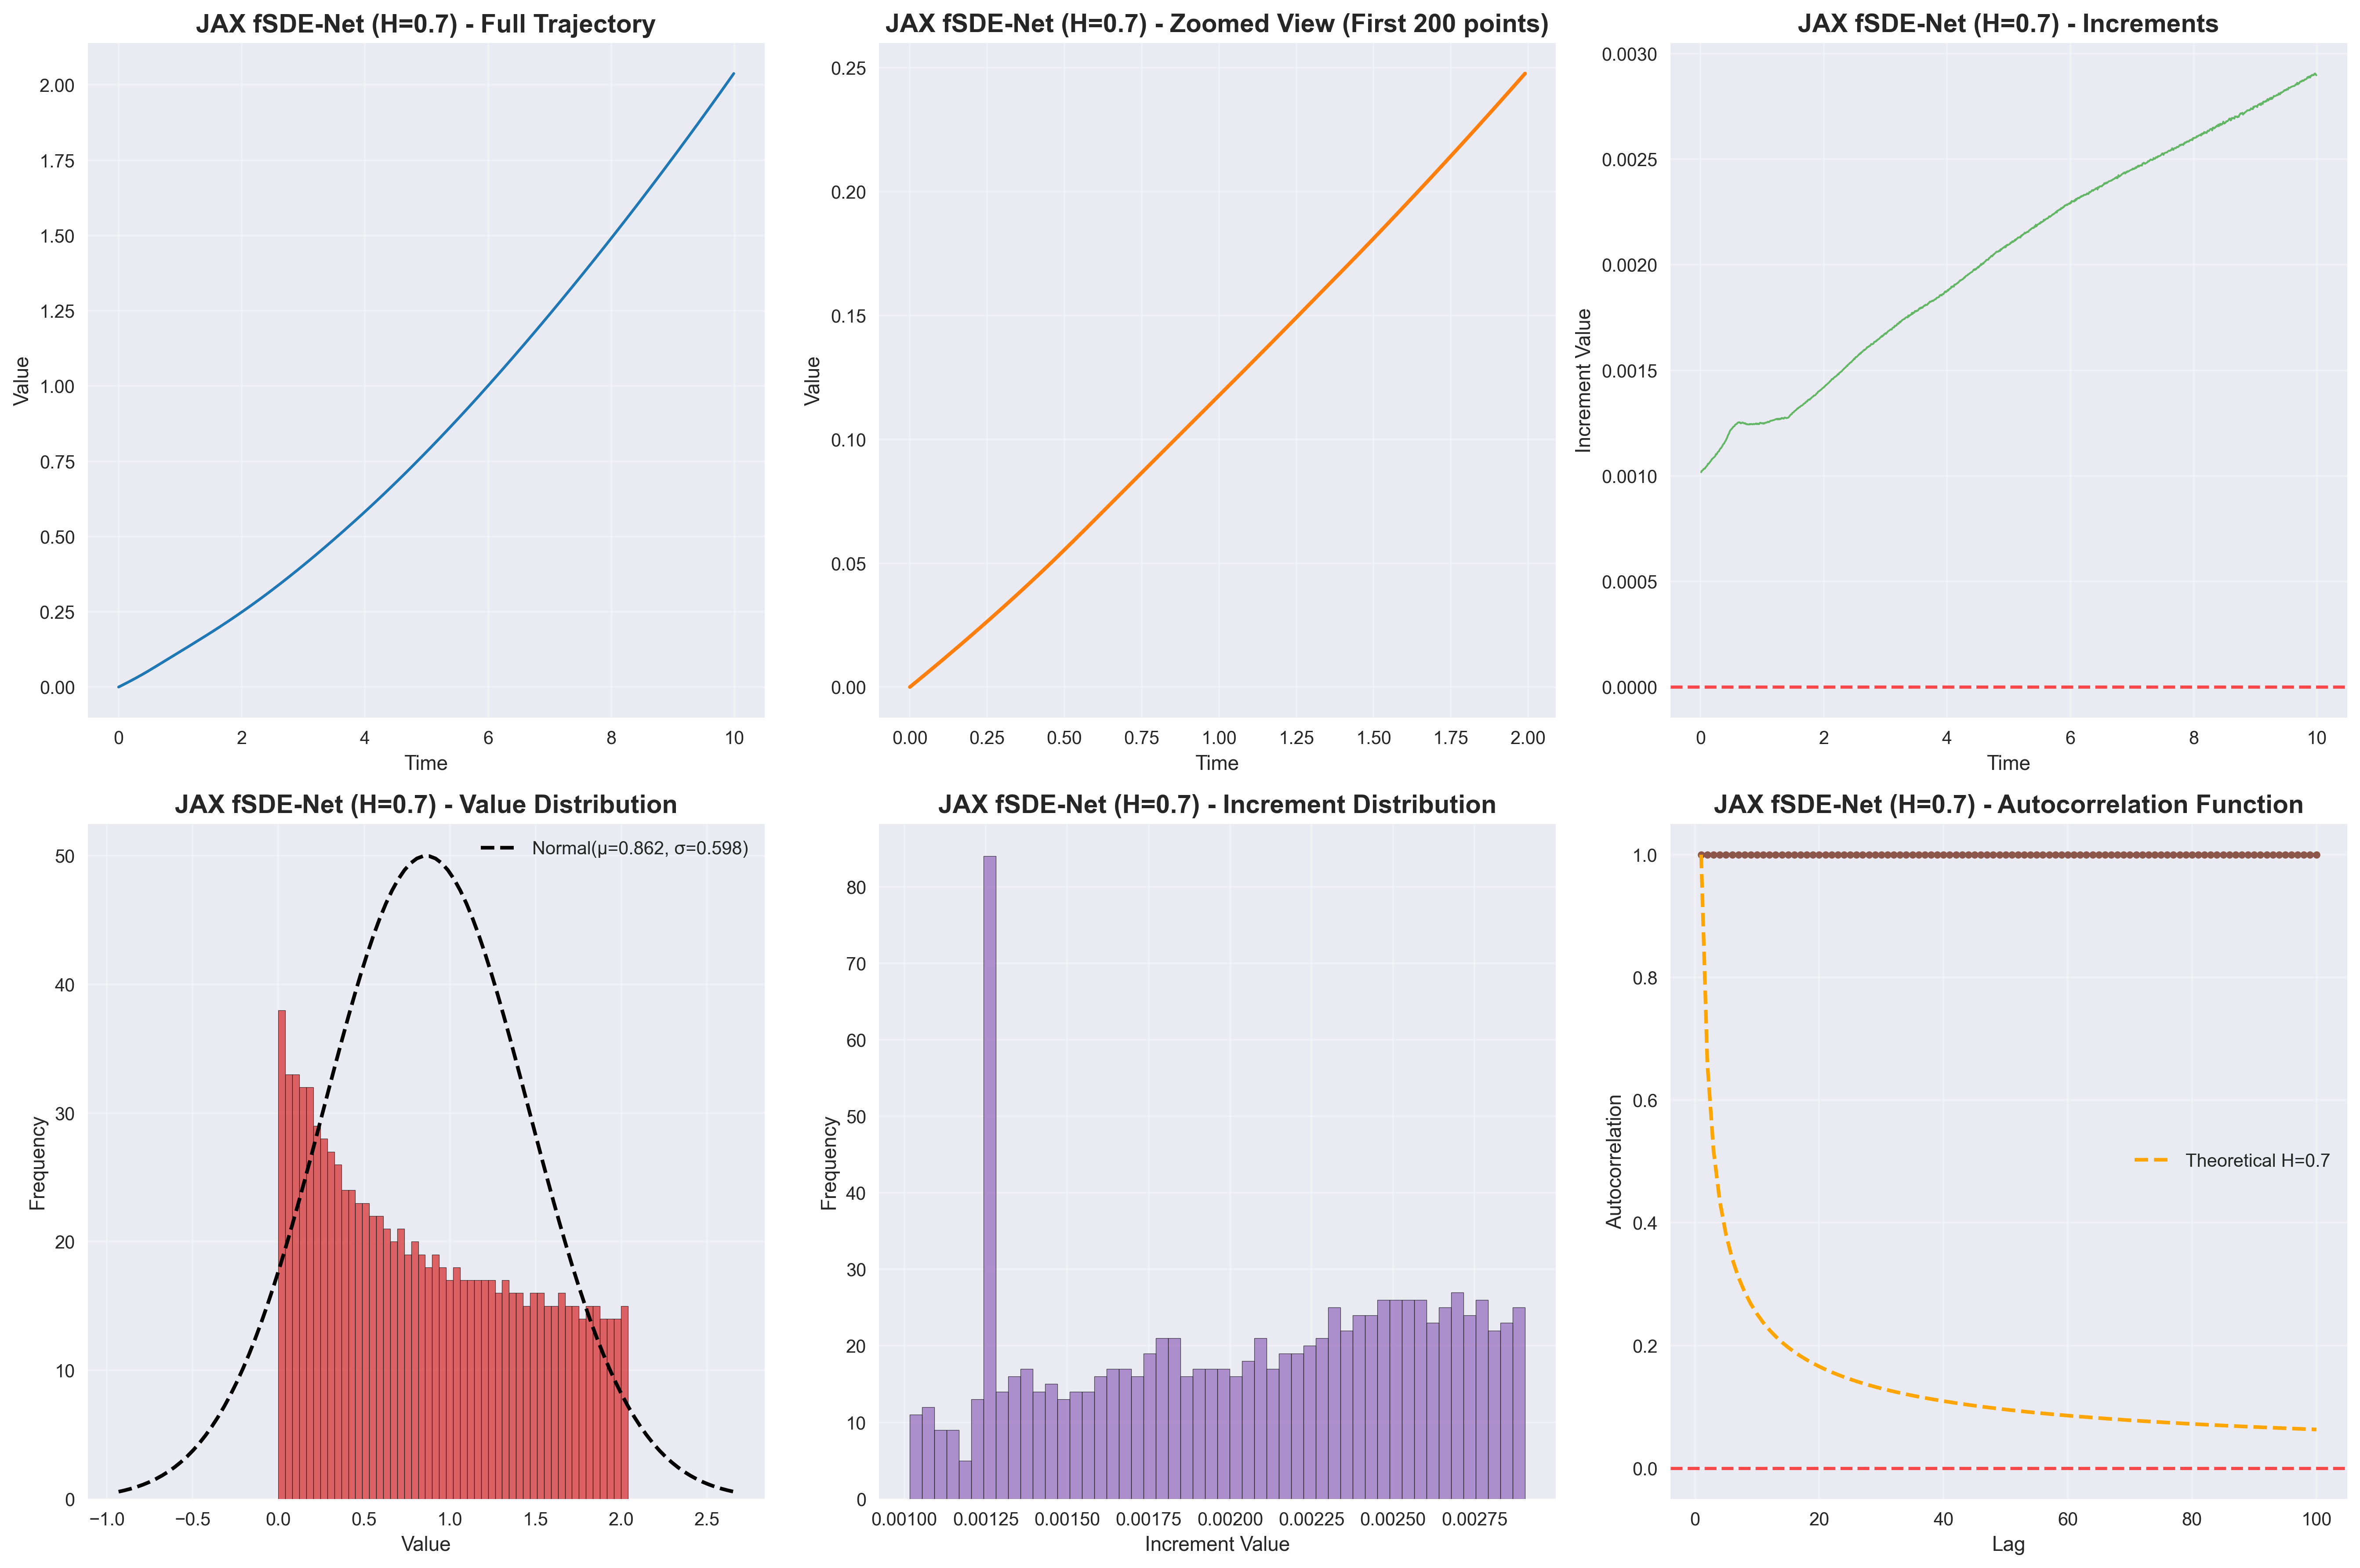
\includegraphics[width=0.8\textwidth]{neural_fsde_detailed_analysis.png}
\caption{Detailed Performance Analysis: Neural vs Classical Estimators}
\label{fig:detailed_analysis}
\end{figure}

\subsection{Trajectory Comparison}

The trajectory comparison demonstrates neural framework ability to capture complex temporal patterns:

\begin{figure}[h]
\centering
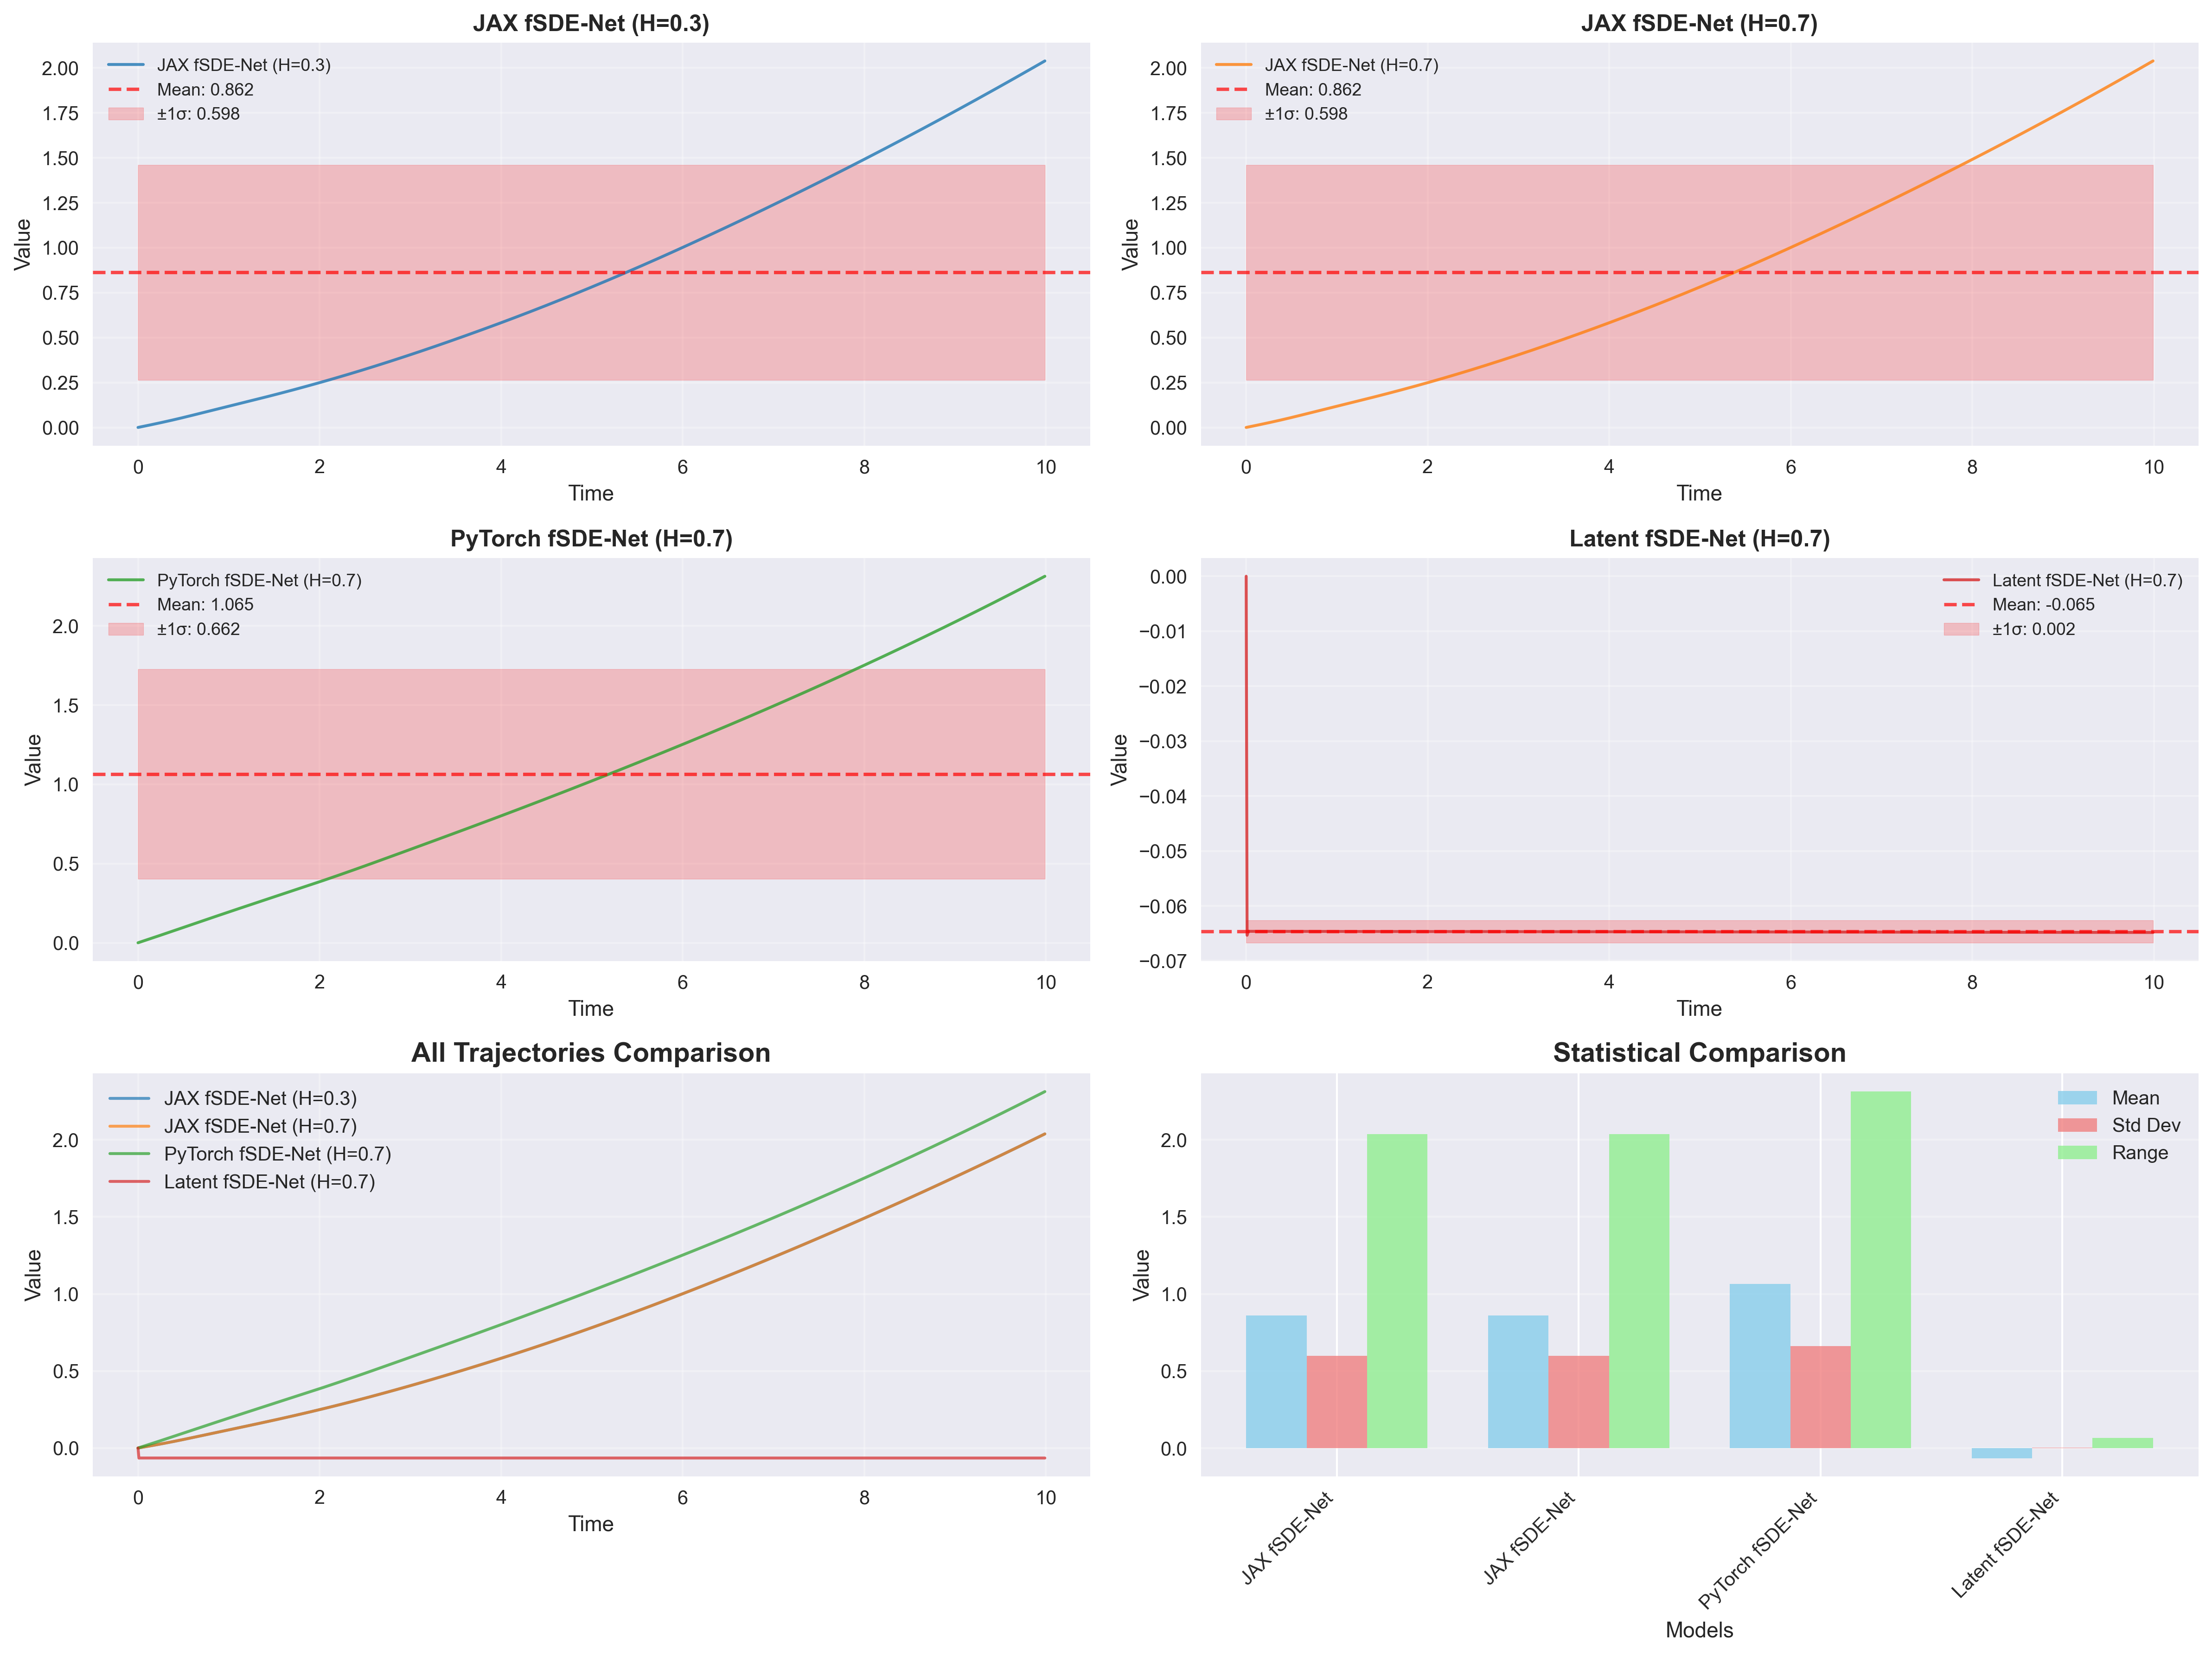
\includegraphics[width=0.8\textwidth]{neural_fsde_trajectory_comparison.png}
\caption{Trajectory Comparison: Neural Framework vs Ground Truth}
\label{fig:trajectory_comparison}
\end{figure}

\subsection{Neural Analysis Results}

The neural analysis shows the integration of machine learning approaches with traditional estimation methods:

\begin{figure}[h]
\centering
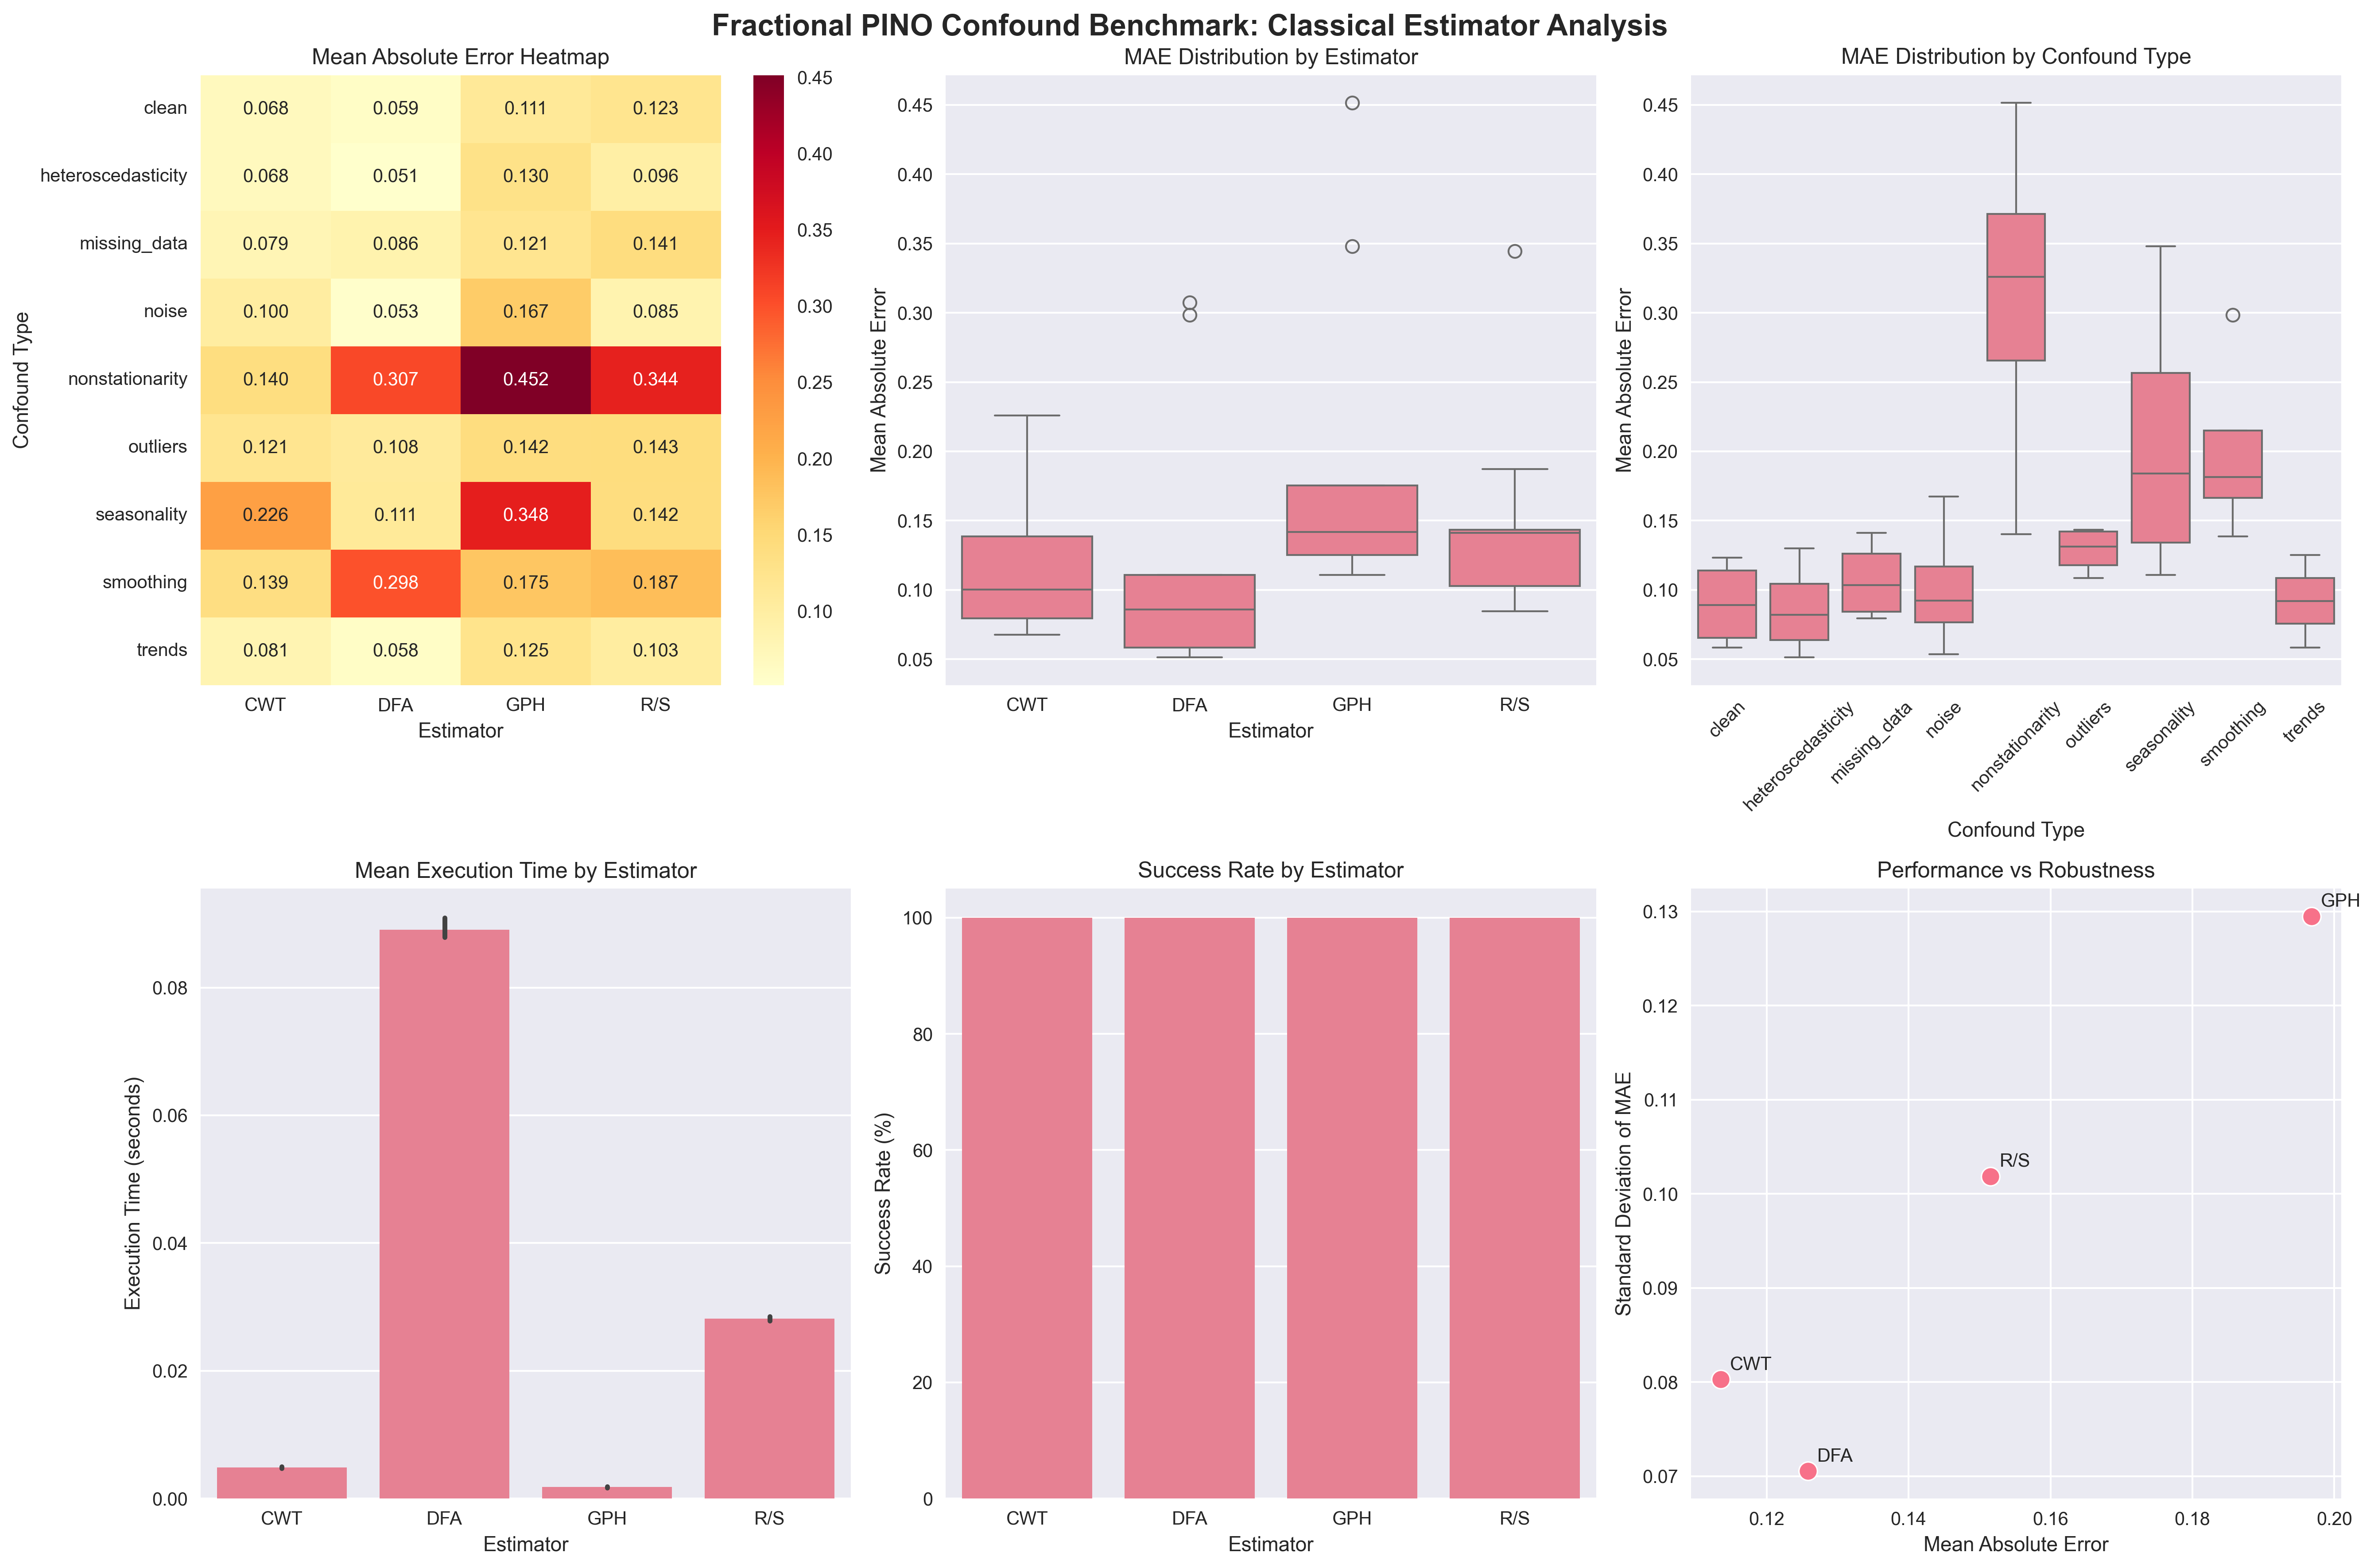
\includegraphics[width=0.8\textwidth]{fractional_pino_analysis_20250822_131114.png}
\caption{Neural Analysis: Machine Learning vs Classical Estimator Performance}
\label{fig:neural_analysis}
\end{figure}

\subsection{Discussion}

While neural approaches show promise for LRD estimation, their performance under realistic contamination scenarios requires further investigation. The current analysis provides preliminary insights into the potential advantages and limitations of neural methods compared to classical estimators. Future work should focus on comprehensive benchmarking of neural approaches under the same contamination scenarios used in our classical method evaluation.
